\documentclass[10pt, aspectratio=169]{beamer}
\usetheme{metropolis}

\usepackage{graphicx}
\usepackage{hyperref}
\usepackage{amsmath}
\usepackage{listings}
\usepackage{xcolor}
\usepackage{qrcode}

\title{Thesis: Development of a University Navigator}
\author{M. Chikishev, M. Sharmanov, A. Andreev, E. Yemelyanov}
\institute{Chelyabinsk State University}
\date{\today}

\begin{document}

\begin{frame}[plain]
	\titlepage
\end{frame}

\begin{frame}{Outline}
	\setbeamertemplate{section in toc}[sections numbered]
	\tableofcontents[hideallsubsections]
\end{frame}

\section{Introduction}

\begin{frame}{Project Rationale}
	\begin{itemize}
		\item Replacement for \href{https://map.csu.ru}{map.csu.ru}
		\item Need for modern 360° panoramic imaging
		\item Discontinued old codebase due to:
		      \begin{itemize}
			      \item Low cost-effectiveness (technical debt)
			      \item Need for modern technology stack
		      \end{itemize}
	\end{itemize}
\end{frame}

\begin{frame}{Project Objectives}
	\begin{itemize}
		\item Cross-platform interactive map editor with 3D imagery
		\item Event and schedule integration, shortest-path routing
		\item Internal communication: ejabberd server + web client
		\item Data import tools (parsers) or manual schedule entry
	\end{itemize}
\end{frame}

\section{Theoretical Framework}

\begin{frame}{Current Challenges}
	\begin{itemize}
		\item No unified secure environment for real-time communication
		\item Decentralized university information resources
		\item Low efficiency of notification channels
	\end{itemize}
	\vfill
	\textbf{Solution:} Aggregate services into a single interface.
\end{frame}

\begin{frame}{Core Development Principles}
	\begin{itemize}
		\item Security, performance, portability, maintainability
		\item Technology stack selected accordingly
		\item Excluded: Python, JavaScript, C\# (performance / architectural mismatch)
		\item Goal: gain experience with high-performance systems
	\end{itemize}
\end{frame}

\begin{frame}{Panoramic Content Visualization}
	\begin{itemize}
		\item Equirectangular projection for 360° images
		\item Implemented with \texttt{three.js} (virtual sphere / cube mapping)
		\item Segmented loading (tiling) for 8K+ images
	\end{itemize}
\end{frame}

\begin{frame}{Routing Fundamentals}
	\begin{itemize}
		\item Weighted directed graph (Poincaré duality)
		\item 3D volumes → nodes, doors → edges
		\item IndoorGML + \texttt{pgRouting} for dynamic subgraph filtering
		\item Shortest path via Dijkstra's algorithm
	\end{itemize}
\end{frame}

\begin{frame}{Distributed Communication Protocols}
	\begin{itemize}
		\item XMPP ~--- open, extensible, XML-based
		\item \texttt{ejabberd} server ~--- fault-tolerant, high concurrency
		\item Provides:
		      \begin{itemize}
			      \item Real-time messaging
			      \item Multi-user conferences
			      \item Notifications
			      \item Isolation of personal social networks
		      \end{itemize}
	\end{itemize}
\end{frame}

\begin{frame}{Information Security}
	\begin{itemize}
		\item \textbf{Shift Left Security} ~--- early vulnerability detection
		\item Go language ~--- memory safety
		\item Defenses:
		      \begin{itemize}
			      \item ORM (SQL injection prevention)
			      \item Anubis (bot protection)
			      \item JWT authorization
			      \item Middleware, distroless containers
			      \item Static analyzers + Quality Gates in CI/CD
		      \end{itemize}
	\end{itemize}
\end{frame}

\section{Practical Implementation}


\begin{frame}{QR Code ~--- Architecture Overview}
	\centering
	\qrcode[height=5cm]{https://github.com/ylnt241/eng-project/blob/main/images/Overview.drawio.png?raw=true}

	\vspace{1em}

	\text{\href{https://github.com/ylnt241/eng-project}{https://github.com/ylnt241/eng-project}}

	\small{Scan to view a high-resolution version of the architecture diagram}
\end{frame}

\begin{frame}{General Architecture Overview}
	\begin{figure}
		\centering
		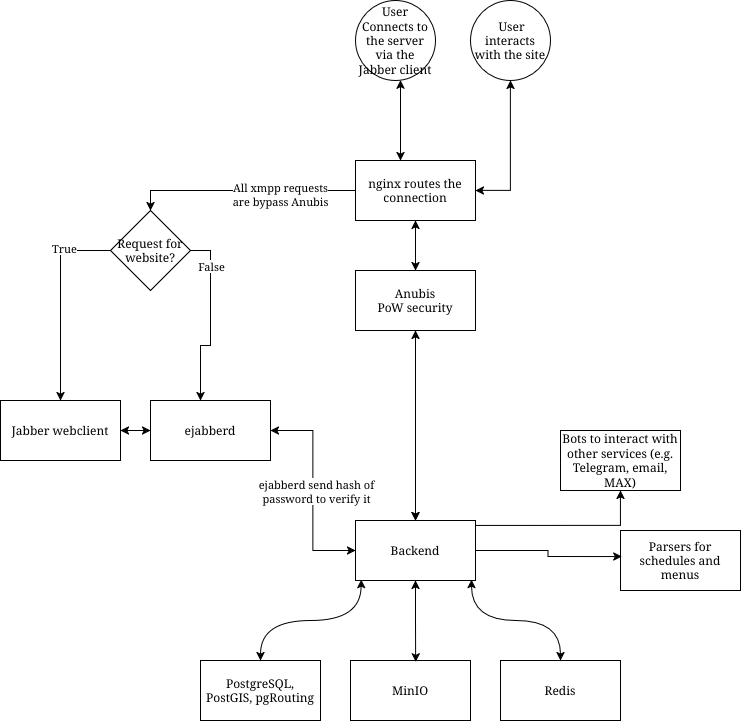
\includegraphics[width=0.7\textwidth, height=0.8\textheight, keepaspectratio]{images/Overview.drawio.png}
		\label{fig:overview}
	\end{figure}
\end{frame}

\begin{frame}{Architectural Principles}
	\begin{itemize}
		\item \textbf{Service Consolidation:} minimize container count
		\item \textbf{Hybrid Monolith:} core logic in a single backend service
		\item \textbf{Stateless Approach:} ready for future clustering
	\end{itemize}
\end{frame}

\begin{frame}{Technology Stack ~--- Core Components}
	\begin{itemize}
		\item \textbf{Networking:} NGINX + Anubis (bot protection)
		\item \textbf{Storage:} PostgreSQL + PostGIS + pgRouting
		\item \textbf{Communication:} Ejabberd + XMPP client
		\item \textbf{Object Storage \& Caching:} MinIO (S3-compatible), Redis
		\item \textbf{External Services:} Python parsers, Go/Python bots
	\end{itemize}
\end{frame}


\begin{frame}{QR Code~--- Backend Structure}
	\centering
	\qrcode[height=5cm]{https://github.com/ylnt241/eng-project/blob/main/images/Backend.png?raw=true}

	\vspace{1em}

	\text{\href{https://github.com/ylnt241/eng-project}{https://github.com/ylnt241/eng-project}}

	\small{Scan to view a high-resolution version of the backend block diagram}
\end{frame}

\begin{frame}{Backend Structure}
	\begin{figure}
		\centering
		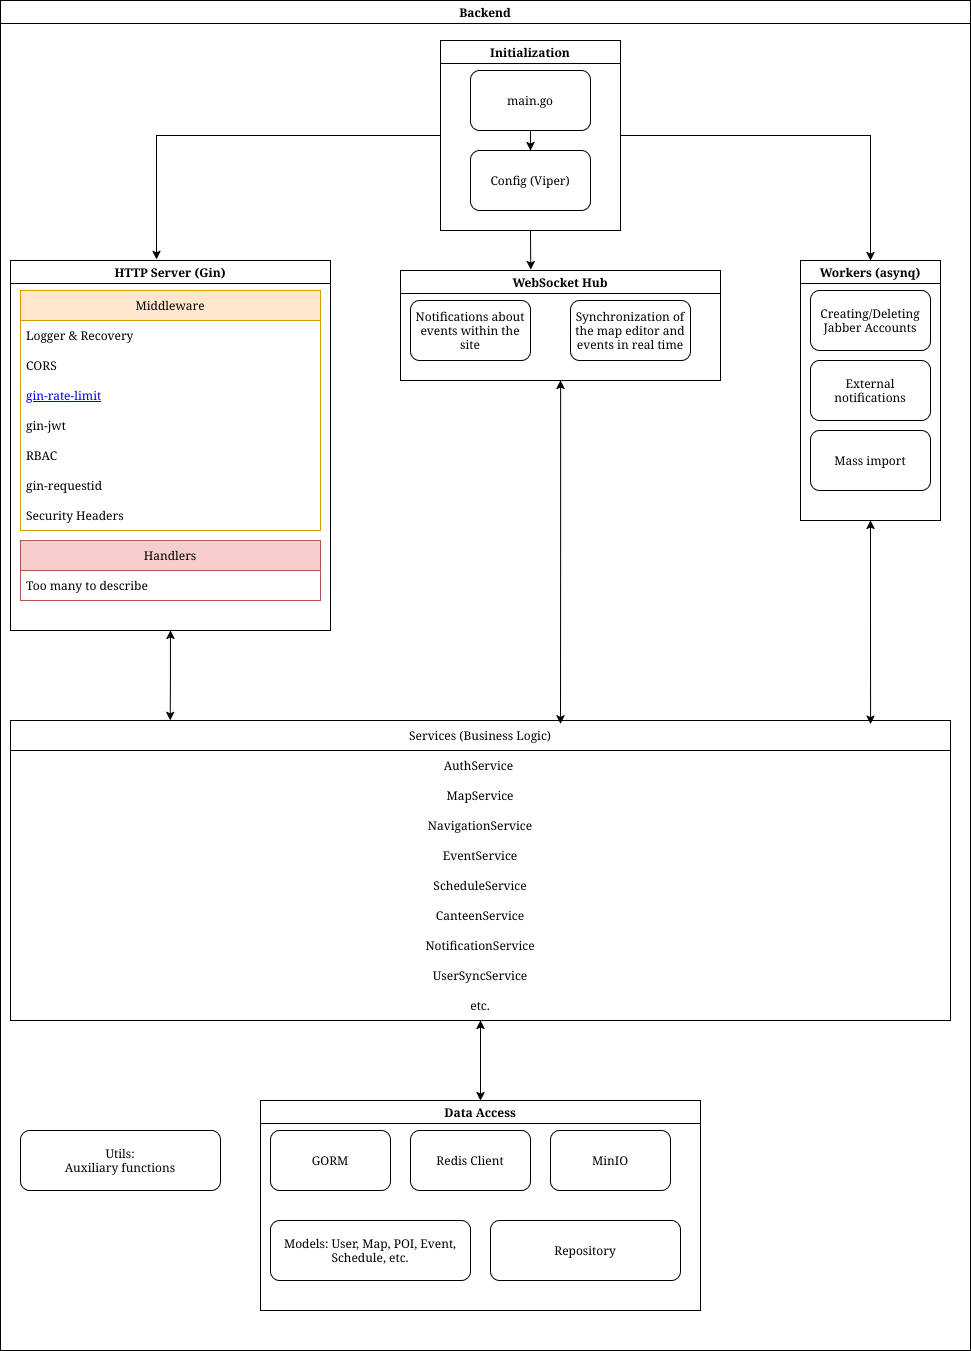
\includegraphics[width=0.7\textwidth, height=\textheight, keepaspectratio]{images/Backend.png}
		\label{fig:backend}
	\end{figure}
\end{frame}

\begin{frame}{Backend Implementation (Go)}
	\begin{itemize}
		\item Multi-layered architecture
		\item \textbf{Initialization:}
		      \begin{itemize}
			      \item Viper for configuration
			      \item Automatic migrations (golang-migrate)
			      \item Redis \& Asynq clients
			      \item Dependency injection
		      \end{itemize}
		\item \textbf{Transport:} Gin framework, WebSocket hub
	\end{itemize}
\end{frame}

\begin{frame}{DevOps and Security}
	\begin{itemize}
		\item \textbf{CI/CD with Jenkins:}
		      \begin{itemize}
			      \item Automated tests on every PR
			      \item SonarQube static analysis + Quality Gates
			      \item Mandatory code review
		      \end{itemize}
		\item \textbf{Containerization:}
		      \begin{itemize}
			      \item Distroless images ~--- minimal attack surface
			      \item Multi-stage builds
		      \end{itemize}
	\end{itemize}
\end{frame}

\begin{frame}{Monitoring and Protection}
	\begin{itemize}
		\item Middleware filtering (SQL injection, XSS)
		\item Anubis + NGINX ~--- block malicious traffic
		\item Ensures availability under limited resources
	\end{itemize}
\end{frame}

\section*{Conclusion}

\begin{frame}{Conclusion}
	\begin{itemize}
		\item Modern navigation ecosystem with 360° panoramas
		\item \textbf{Key achievements:}
		      \begin{itemize}
			      \item Go-based high-performance backend
			      \item pgRouting + graph model for indoor navigation
			      \item Shift Left Security, distroless containers
			      \item Stateless, scalable architecture
		      \end{itemize}
		\item Improves digital interaction for students and staff
	\end{itemize}
\end{frame}

\begin{frame}{The end.}
	\centering
	\vfill
	\Large{Thank you.}
	\vfill
\end{frame}

\end{document}
